\documentclass[10pt]{article}
\usepackage{fontspec}
\setmainfont[Ligatures=TeX]{Didot}
\usepackage[utf8]{inputenc}
\usepackage[papersize={17in, 11in}]{geometry}
\usepackage[absolute]{textpos}
\TPGrid[0.5in, 0.25in]{23}{24}
\usepackage{palatino}
\parindent=0pt
\parskip=12pt
\usepackage{nopageno}
\usepackage{graphicx}
\graphicspath{ {./images/} }
\usepackage{lilyglyphs}
\usepackage{amsmath}
\begin{document}

\vspace*{0.5\baselineskip}

\begin{center}
\huge FOREWORD
\end{center}

\begin{center}
Cthar is a hebrew word, meaning "to hide" or "to disassemble."\\
\phantom{text} \hfill (G.R.E.)
  \end{center}
  
\vspace*{3\baselineskip}

\begin{center}
\huge PERFORMANCE NOTES
\end{center}

\begin{center}
\pmb{Microtones}:
\end{center}

\begin{center}
\includegraphics[width=0.5\textwidth]{microtones.png}
\end{center}

\begin{center}
Accidentals apply only to the pitch which they immediately precede.
\end{center}

\pmb{Bow Position Staff} 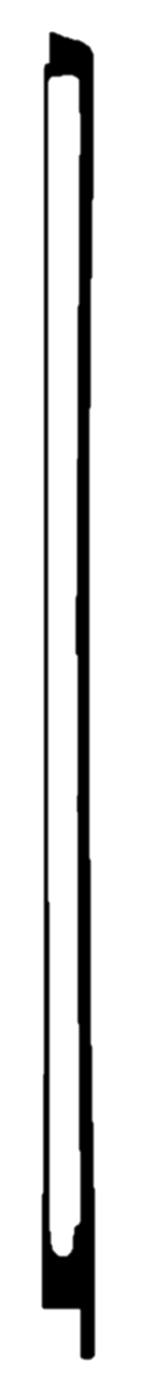
\includegraphics[height=0.025\textheight]{bow_position_tablature.eps}: The middle staff for each instrument notates the horizontal contact point at which the bow touches the string. These positions are written as fractions where \( \frac{0}{1} \) represents $au \ talon$ and \( \frac{1}{1} \) represents $punta \ d'arco$.

\vspace*{8\baselineskip}

\begin{center}
c.10'
\end{center}

\end{document}